\chapter{Introduction}

\blindtext
 Eine Testformel,
\begin{equation}
  E=m c^2,
\end{equation}
mit Energie $E$, Masse $m$ und Lichtgeschwindigkeit $c$.
\blindtext
\begin{equation}
  a^2 - a^2 = a^2 - a^2
\end{equation}
\blindtext
\begin{equation}
  b^2 - b^2 = b^2 - b^2
\end{equation}
\begin{equation}
  c^2 - c^2 = c^2 - c^2
\end{equation}
\blindtext
\begin{gather}
  b^2 - b^2 = b^2 - b^2\\
  c^2 - c^2 = c^2 - c^2
\end{gather}

\section{Section}
\Blindtext[3]

\subsection{Subsection}
\Blindtext[1]\cite{MUNE09}

\subsubsection{Subsubsection}
\Blindtext[2]

\begin{figure}[tb]
    \centering
    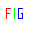
\includegraphics[width=0.98\textwidth]{fig/test.png}
    \caption{Test figure.}
    \label{fig:test}
\end{figure}

See Figure~\ref{fig:test}.

\Blindtext
